\documentclass[10pt,a4,oneside]{article}
\usepackage{a4wide}
\usepackage{graphicx}

\begin{document}
\begin{titlepage}
\begin{center}

\includegraphics[width=40mm]{figs/earth}
\vfill
\textbf{\huge Milestone 4 Plan}\\ \textit{} \\ \textit{} 
\textit{for} \\ \textit{} \\ \textit{} 
\textbf{\huge Subgroup 1}\\ \textit{} \\ \textit{}
\vfill
\textbf{Alex Egan \\ Filimoni Lutunaika \\ George Sainsbury \\ Xiaodong Cui}
\end{center}
\end{titlepage}
 


\newpage

\tableofcontents

\[----\]

\paragraph{}

\listoffigures
 
\newpage

\section{Introduction} 
 
\subsection{Purpose and Scope}

\label{subsec:purpose-and-scope}
 
Milestone 4 follows on from the development tasks undertaken during Milestones 1 to 3.
For the current development sprint, Subgroup 1 will proceed with developing solutions 
to the following Tickets, which were initially investigated in Milestone 3:

\subsubsection*{ Ticket 131 - Use real disk usage instead of byte size throughout the web application}

\noindent We are now gathering disk space usage (number of occupied 512-byte blocks) 
along with the size of each file. This is a more precise metric for 
determining where disk space is used, which probably is Earth's main purpose at this time. 
Therefore, the GUI should use this value instead in all situations. (Maybe it should be 
configurable in earth-webapp.yml.) 

\subsubsection*{ Ticket 174 - Look into making Earth release a gem}

\noindent It would allow us to automatically deal with the dependencies such as:

\begin{itemize}
\item the gems:
  \subitem rcov
  \subitem rails
  \subitem postgres 
\end{itemize}
 
\subsubsection*{ Ticket 186 - Remove feature for Earth daemon}

\noindent The remove command for earthd needs to be implemented. It should 
remove a directory so that it is no longer monitored on the local host. Also, 
it should allow for historical tracking of files so that it can be seen where 
files have been deleted. \\

\noindent In addition, Subgroup 1 is also planning to investigate and fix the following Ticket:

\subsubsection*{ Ticket 75}
\noindent Implemented listing by either name OR (with a slight modification) size.
Future enhancement should consider dynamic sorting wherein clicking the 
field title sorts the record according that particular field.


\subsection{Plan Review}
 
\noindent This plan will be reviewed at the end of the Milestone 4 development 'sprint'. However,
it will be updated if there is a radical change to the requirements of any Milestone 4 task. 
The changes can be made by any of the Subgroup member who should then inform the Subgroup leader 
about these changes. However, significant changes that have a system-wide effect will be deferred 
to the next milestone to minimize any disruption to the other tasks of the current milestone.

\newpage

\section{Organisation for Milestone 4}
 
\label{sec:g1org}

\subsection{Task Allocations}

Tasks for Milestone 4 are being allocated as follow:

\subsubsection{Ticket 75: Sort by name or size}

\paragraph{Description}
Alex is being allocated this task which enables dynamic sorting of 
listed directories and files under the navigation tab. The Group had initially investigated
and implemented a solution that sorted the listing either by name or (with a minor
modification) size.

\paragraph{Subtasks}
\noindent
\begin{enumerate}
\item Design and code the dynamic sorting of record listing. (7hrs)
\item Test and integrate solution to the Subgroup 1 codebase. (2hrs)
\item Update the Earth Trac system. (1hr)
\end{enumerate}

\paragraph{Total Time Estimate} 10hrs

\subsubsection{Ticket 131: Use real disk usage instead of byte size}

\paragraph{Description}
Cui is being allocated this task which involves modifying the web interface 
to display the real disk usage instead of the current byte size values. He
had implemented some highly fragmented solutions in Milestone 3. He is 
expected to produce a relatively modular and generic implementation during
this current Milestone (4).

\paragraph{Subtasks}
\noindent
\begin{enumerate}
\item Investigate potential solutions. (24hrs) 
\item Design and code the most efficient solution. (40hrs)
\item Test and integrate solution to the Subgroup 1 codebase. (8hrs)
\item Update the Earth Trac system. (1hr)
\end{enumerate}

\paragraph{Total Time Estimate} 73hrs

\subsubsection{Ticket 174: Creating the Earth Gem}

\paragraph{Description}
George is being allocated this task which involves implementing 
a Gem for the Earth web application. This will be a continuation
of the task he undertook during Milestone 3 wherein he investigated 
and partly implemented the Earth Gem.
\\This revision of the Earth Gem will be able to be installed from, include
the documentation files and he will test the installation via a web source.
\\The availability of this 
Gem will have a significant impact on the productivity of developers 
as less resources (time) is required to modify and configure the Earth
application.

\paragraph{Subtasks}
\noindent
\begin{enumerate}
\item Refamiliarise with the ruby gem specification syntax and reassess progress from Milestone 3. (2hr)
\item Code the implementation of the gem. (1hr)
\item Test whether the implementation of the gem can install and contains all the relevant files. (3hrs)
\item Try to upload the gem to a location so "gem install" can be used. (4hrs)
\end{enumerate}

\paragraph{Total Time Estimate} 10hrs
 
\subsubsection{Ticket 186: Remove Feature of Earth Daemon}

\paragraph{Description}
Fili is being allocated this task which entails implementing the 
Earth remove feature. This task was investigated by the Subgroup in Milestone 3
and had to be deferred due to its relatively heavy resource requirements.

\paragraph{Subtasks}
\noindent
\begin{enumerate}
\item Investigate the existing add feature of the daemon. (8hrs)
\item Identify the relevant components of the remove feature. (16hrs)
\item Design and code an effective implementation of the remove feature. (40hrs)
\item Test and integrate solution to the Subgroup 1 codebase. (16hrs)
\item Update the Earth Trac system. (1hr)
\end{enumerate}

\paragraph{Total Time Estimate} 81hrs

\newpage
 
\subsection{Scheduling}

\paragraph{} 
The milestone subtasks are presented in a gantt chart shown in Figure \ref{fig:m4gantt} below. 
The gantt chart shows the scheduling of the subtasks for each Ticket and the overall completion
schedule of Milestone 4. 

 
\begin{figure}[h!]
\begin{centering}
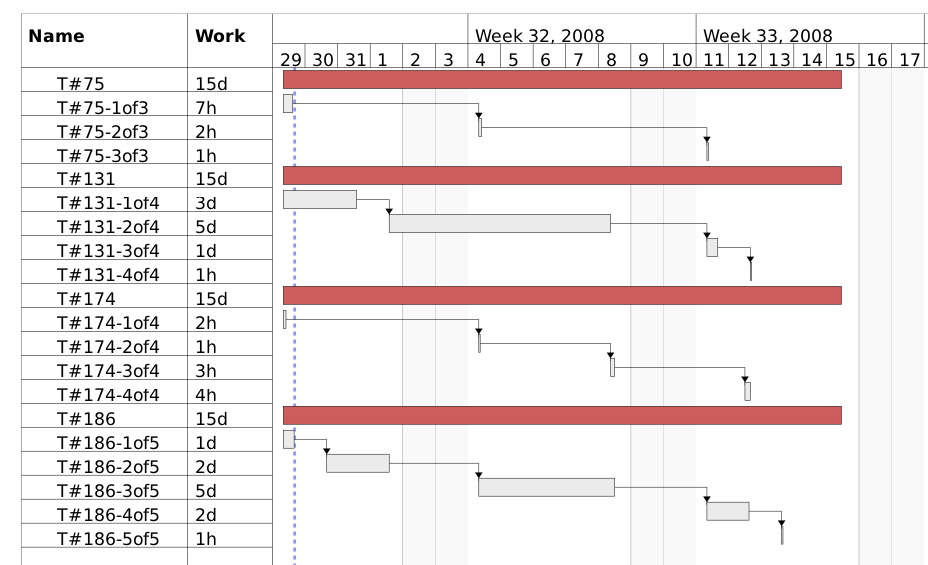
\includegraphics[width=150mm]{figs/m4gantt}
\end{centering}
\caption{Milestone 4 Gantt Chart}
\label{fig:m4gantt}
\end{figure}

\newpage

\subsection{Resource Allocation}
 
\paragraph{}
As described in Section \ref{subsec:purpose-and-scope}, resources (developers) will be allocated to 
each task as follow:
 
\begin{itemize}
  
\item \textbf{Ticket 75:} Alex Egan \\

\item \textbf{Ticket 131:} Xiaodong Cui \\ 
 
\item \textbf{Ticket 174:} George Sainsbury \\
 
\item \textbf{Ticket 186:} Filimoni Lutunaika \\
 
\end{itemize}
 
If a task is completed early, or it is noted that less people are required to complete a task on schedule, they will be reallocated to other tasks.\\
 
\subsection{Source Control}

\subsubsection{Task Completion Criteria}

\noindent To ensure the successful integration of each allocation tasks into the Subgroup repository, the member responsible will have to make sure that at least one of the other Subgroup members can successfully duplicate the end results or outcome of the task.

\paragraph{}
\noindent Upon satisfying the above requirement, the member responsible can then make a pull request to the Subgroup's gitHub leader to upload the solution onto the Subgroup's git repository for the actual integration testing of the Subgroup's collective solutions. 


\subsubsection{Git Repository Process}

\noindent Each Subgroup member is expected to follow the git repository procedures outlined in the \emph{Repository Process Document for Earth}.
 

\subsubsection{Testing Process}
\noindent Each Subgroup member is expected to follow the testing process procedures outlined in the \emph{Testing Process Document for Earth}.


\subsection{Administration}

In addition to the assigned tasks for this Milestone, the roles of Git Leader and Documentation Person will be rotated amongst the Subgroup 1 members at every milestone. This will help to ensure that each member gets a chance to take on extra responsibilities with the view of broadening their individual skills as a software developer.

\subsubsection{Git Leader}

For Milestone 4, Cui will be in charge of managing the repository for Subgroup 1. This includes ensuring that the Milestone 4 solutions undergo integration testing before being committed onto the Subgroup 1 repository.


\subsubsection{Documentation Person}

For Milestone 4, Fili will oversee the documentation requirements for Subgroup 1, which mainly includes setting meeting agendas and organising progress update meetings.

\newpage

\section{References}
 
Sommerville, I. \textit{Software Engineering}, 8th Edition,  Addison-Wesley, 2007\\
\newline
Earth Project, \textit{Ticket 75} Retrieved from \emph{http://open.rsp.com.au/projects/earth/ticket/75} on 29/07/2008.\\
\newline
Earth Project, \textit{Ticket 131} Retrieved from \emph{http://open.rsp.com.au/projects/earth/ticket/131} on 29/07/2008.\\
\newline
Earth Project, \textit{Ticket 174} Retrieved from \emph{http://open.rsp.com.au/projects/earth/ticket/174} on 29/07/2008.\\
\newline
Earth Project, \textit{Ticket 186} Retrieved from \emph{http://open.rsp.com.au/projects/earth/ticket/186} on 29/07/2008.\\
\newline
Egan, A and Bamogaddam, M.,\textit{Testing Process Document for Earth} Egan, A and Bamogaddam, M., First Edition, 2008.\\
\newline
Egan, A and Bamogaddam, M.,\textit{Repository Process Document for Earth}  First Edition, 2008.\\

\paragraph{}

\[ END\]
\end{document}
